% Generated from retained results by build_report.py. Official class unchanged.
\documentclass{COMPXXXX}
\usepackage[OT1]{fontenc}
\usepackage{times}
\usepackage{amsmath,amssymb,graphicx,array,capt-of,balance}
\usepackage[hidelinks]{hyperref}
\begin{document}
\title{Potential shifting under corrupted guidance\\A controlled tabular reconstruction}
\author{Student ID: 001388739}
\maketitle
\bibliographystyle{COMPXXXX}
\begin{abstract}
This study reconstructs potential shifting under unresolved normalisation and cutoff details and evaluates a stationary graph-smoothing modification. The frozen design retains all initialisations and both potential scales. Across 1,500 core configuration runs, smoothing shifted guidance changes mean checkpoint original-task return by +0.0113 (95\% paired seed-block bootstrap interval [+0.0069, +0.0170]). The gain is concentrated in unit-scaled, strongly corrupted conditions. Another 300 source-like runs expose scale sensitivity. All failed conditions are retained; exact reproduction, general improvement and algorithmic novelty are not claimed.
\end{abstract}

\section{Problem and related research}
Sparse rewards make navigation learning sensitive to exploration and initial values. The question is whether a fixed local smoothing of corrupted guidance improves the finite-budget performance of the potential-shifting construction of M{\"u}ller and Kudenko~\cite{mueller2025}. This is a study of that method under declared reconstructions, not an attempt to match every published result.

Potential shaping has a policy-invariance foundation~\cite{ng1999}; its static form is also related to potential-informed Q initialisation~\cite{wiewiora2003}. Those properties concern the defined task and update conditions, not guaranteed acceleration. Incorrect guidance is not an unexplored topic: M{\"u}ller, Berg and Kudenko~\cite{plans2025} already address incomplete and incorrect symbolic plans with exponential plan-based shaping. Here, the representation is a frozen scalar field, and the contribution is a controlled shift/smoothing ablation, not a new claim about solving imperfect plans. Graph diffusion is established~\cite{kondor2002}; the proposed composition uses one simple Laplacian step rather than a new diffusion theory.

\begin{table*}
\centering
\begin{tabular}{lllrrrr}
\hline
Reward & Cutoff & Scale & Unshaped MCR & PBRS MCR & Shifted MCR & Shifted final success\\
\hline
G & B & L & 0.0000 & 0.0000 & 0.0000 & 0.000 \\
G & B & U & 0.0000 & 0.0261 & 0.0782 & 1.000 \\
G & Z & L & 0.0000 & 0.0000 & 0.0000 & 0.000 \\
G & Z & U & 0.0000 & 0.0261 & 0.0782 & 1.000 \\
S & B & L & -19.9999 & -19.9999 & -19.0641 & 0.953 \\
S & B & U & -19.9999 & -19.9999 & -18.5262 & 1.000 \\
S & Z & L & -19.9999 & -19.9999 & -19.0603 & 0.987 \\
S & Z & U & -19.9999 & -19.9999 & -18.5262 & 1.000 \\
\hline
\end{tabular}
\caption{Complete source-like factor groups, averaged over three Q initialisations and five paired seeds per row (15 configuration runs, not 15 independent seeds). G: goal reward; S: step reward. B: bootstrap; Z: zero endpoint/no bootstrap at cutoff. L: literal scale; U: additional factor $1/32$. MCR is discounted original return, so larger is better within each reward. Final success averages ten last-checkpoint evaluation episodes per run. The same unshaped runs are reused as references across scale rows; they are not extra observations. Full initialisation-level outcomes and all episodes accompany the code.}
\label{tab:source}
\end{table*}
\begin{figure*}[tp]
\centering
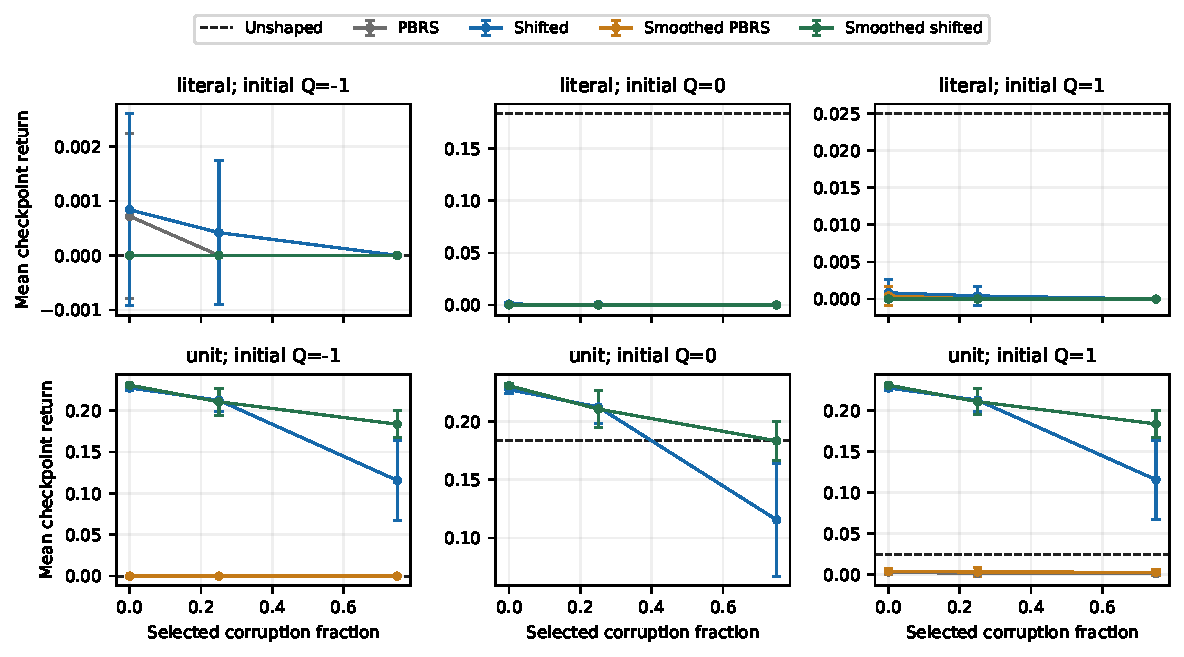
\includegraphics[width=\textwidth]{../analysis/figures/core_comparison.pdf}
\caption{Core learning efficiency by scale, initial Q and selected corruption fraction. Lines show MCR averaged over two fixed maps and ten paired seed blocks; error bars are the standard deviation of the map-averaged block values. Higher is better. Each run uses 50,000 training transitions and fifty ten-episode greedy evaluations, cap 250. The dashed unshaped reference reuses the same runs across irrelevant scale/corruption conditions. Both normalisations and all initialisations are shown; literal and unit panels need not share a useful performance range.}
\label{fig:core}
\end{figure*}
\section{Methods and controls}
The simulator has four deterministic cardinal actions, boundary/wall self-loops, corner start/goal, and a 250-transition collection cap. Off-grid actions consume a step. Goal termination takes priority at a simultaneous cap. Goal rewards are 1 on entry and 0 otherwise; the alternative step-reward condition gives $-1$ on every transition. States encode position only: 625 allocated positions in the source-like grid and 100 in each core grid. No time-augmented learner is implied.

For Manhattan distance $d$ and its maximum $D$, let $h=1-d/D$. The two explicit reconstructions are $E_L=32^h$ and $E_U=32^{h-1}$ at non-terminal states, with terminal values zero. The extra factor $1/32$ is scientifically material because task rewards are not rescaled. The paper describes normalised distance and base 32 but does not unambiguously specify their complete combined pipeline. Grid conventions, tie-breaking, author seeds and exact cutoff updates are also not recovered. Both scales are retained instead of silently selecting the favourable one.

The non-terminal shift and shaping rule are
\begin{equation}
\begin{split}
b&=(1-\gamma)Q_0-r_\infty,\\
\Psi_b(s)&=E(s)+b/(\gamma-1),\\
R'&=R+\gamma\Psi_b(s')-\Psi_b(s),
\end{split}
\label{eq:shift}
\end{equation}
with the \emph{complete} terminal potential overridden to zero. Equation~\ref{eq:shift} changes non-terminal shaping rewards by $b$; terminal transitions do not receive that same constant change. Selecting only a poor $Q_0$ would bias the comparison, so all $Q_0\in\{-1,0,1\}$ remain. In the goal/$Q_0=0$ condition, the prescribed shift is zero: 260 saved pairs agree exactly across the full matrices.

\subsection{Stationary method modification}
Corruption permutes selected fractions $f\in\{0,.25,.75\}$ of non-terminal values, using the same frozen instance across paired methods. It preserves the value histogram; fixed points mean actual changed fraction can differ from $f$. The extension applies
\begin{equation}
\widetilde E=(I-L/4)E
\label{eq:smoothing}
\end{equation}
before the same shift, where $L$ is the undirected non-terminal grid Laplacian. The single synchronous step has fixed strength one. Equation~\ref{eq:smoothing} preserves the non-terminal mean and cannot expand the range, but can flatten useful gradients. Goal and wall nodes are excluded. It uses known simulator adjacency, not BFS distances, rollouts or evaluation outcomes. All shaping constructors have the same graph access; applicability without that model is not established.

Directional consistency is measured offline against BFS-distance changes on a fixed, uniformly weighted set of legal non-terminal edges. Self-loops, equal-distance and terminal edges are excluded; potential ties are recorded separately. This diagnostic is not a learner input. The corruption also changes spatial smoothness, so this experiment cannot identify a universal effect of a single reliability scalar.

\subsection{Cutoffs, invariance and evaluation}
The primary protocol bootstraps at external non-goal truncations and retains the next potential. True goal termination uses zero next potential/value. The source-like sensitivity condition instead zeros the endpoint potential and suppresses bootstrapping at the cap. It reflects the paper's discussed cutoff behaviour without claiming exact code recovery. Modern continuing-task truncation handling~\cite{gymnasium} must not be called identical to the latter. The capped position-only variant is not a fully observed stationary finite-horizon MDP; ordinary stationary policy-invariance claims are restricted to the underlying goal-terminated bootstrap task. A time-indexed alternative would have 156,875 states and was not introduced as an inconsequential correction.

Static shaping telescopes to a start-state constant under appropriate boundaries, without guaranteeing finite-budget convergence or every capped metric. Training uses $\alpha=.1$, fixed $\epsilon=.05$, $\gamma=.95$ and uniform greedy tie-breaking. Separate recorded PCG64 streams isolate training, corruption and evaluation; evaluation cannot update Q or consume training randomness.

\section{Executed experiments and results}
The source-like suite has 300 distinct configuration runs: open $25\times25$, both rewards, two cutoff rules, two scales, three initialisations and five paired seeds; irrelevant duplicates of unshaped runs are removed. Each run trains for 250,000 steps and evaluates ten $\epsilon=.05$ episodes every 250 steps. These are selected reconstruction settings, not proof of full replication.

The core suite has 1,500 runs over open and detour $10\times10$ maps, both scales, all three corruption levels and initialisations, and ten paired seed blocks. It compares unshaped Q-learning, PBRS, shifted PBRS, smoothed PBRS and smoothed shifted PBRS. Each run trains for 50,000 steps and evaluates ten greedy episodes every 1,000 steps. All evaluation episodes have cap 250. The detour map has 18 walls; the maps' shortest paths are 18 and 36 steps.

The primary per-run metric is mean checkpoint discounted original return (MCR), averaging all scheduled evaluations, not a post-hoc convergence threshold. The prespecified extension contrast is smoothed shifted minus shifted MCR. Fixed map/scale/corruption/initialisation cells are averaged within each seed first; the ten block means, not millions of episodes, are the independent resampling units. Intervals use 10,000 percentile bootstrap resamples and are conditional on this finite design. Factor-specific summaries are descriptive rather than an uncorrected collection of significance claims.



In Table~\ref{tab:source}, goal-reward shifted runs have final mean success 1.000 under U and 0.000 under L. Large positive potentials create negative goal-entry shaping terms when terminal potentials are zero, changing early incentives. These reconstruction outcomes do not refute the published method or resolve its normalisation ambiguity.



\par\medskip
\noindent\begin{minipage}{\linewidth}\tabsize
\centering
\begin{tabular}{@{}p{.47\linewidth}r p{.31\linewidth}@{}}
\hline
Paired MCR contrast & Mean & 95\% interval\\
\hline
Shift minus PBRS & +0.0614 & [+0.0577, +0.0644] \\
Smooth shift minus shift & +0.0113 & [+0.0069, +0.0170] \\
Smooth PBRS minus PBRS & +0.0040 & [+0.0024, +0.0060] \\
Extension: literal only & -0.0004 & [-0.0008, +0.0000] \\
Extension: unit only & +0.0231 & [+0.0143, +0.0341] \\
Extension: 25\% corruption & -0.0011 & [-0.0053, +0.0036] \\
Extension: 75\% corruption & +0.0339 & [+0.0216, +0.0505] \\
\hline
\end{tabular}
\captionof{table}{Absolute differences in discounted original-task MCR, not accuracy percentages. Positive extension values favour smoothing. Each interval resamples ten seed-block means after equal weighting of the fixed factors in its stated subset. The pooled extension contrast is primary; scale/corruption subsets expose heterogeneity and are descriptive.}
\label{tab:contrasts}
\end{minipage}\par\medskip

Figure~\ref{fig:core} and Table~\ref{tab:contrasts} show a pooled extension effect of +0.0113, but unit scale accounts for the positive gain (+0.0231); the literal-scale contrast is -0.0004 with an interval touching zero. At 25\% selected corruption the interval spans zero, whereas the 75\% condition has a larger positive contrast. This supports a conditional benefit in this design, not a general denoising or policy-improvement claim. Zero final-checkpoint successes occur in 201 of 360 shifted core runs and 189 of 360 smoothed shifted runs; failure is not removed from averaging.

\section{Critical review and limitations}
\subsection{Comparison with the selected paper}
M{\"u}ller and Kudenko's Figure~3 and Section~6.2.1~\cite{mueller2025} report strong dependence on matching bias to initial Q, and cutoff-related failures under negative step rewards. Our unit-scale goal results agree qualitatively with the usefulness of the matched shift, while literal-scale failure prevents a scale-independent agreement claim. The step-reward reconstruction mostly succeeds at its final checkpoint; it does not reproduce the reported failure pattern. We did not retain training trajectories sufficient to diagnose oscillation at previous cutoff states, so that mechanism cannot be claimed from aggregate returns.

These results are an \emph{empirical reconstruction}: selected settings and the shift equation are implemented under explicit missing-detail assumptions. \emph{Qualitative agreement} concerns a direction or dependency; \emph{exact reproduction} would require the same construction, transitions, cutoff updates, seeds and matching outputs. Those conditions are unmet. The paper plots evaluation episode lengths with standard errors; our primary statistic is checkpoint-averaged discounted return. Our comparison includes zero and prescribed bias, not the paper's complete bias sweep. No author raw data or complete implementation was available to this analysis; no speedup ratio, curve-error measure or numerical superiority over the published results is inferred.

\subsection{Four-arm interaction: exploratory analysis}
Table~\ref{tab:arms} retains all four shaping arms. Smoothing without shifting changes MCR by +0.0040; the primary smoothing gain with shifting is +0.0113. A reviewer-requested \emph{post-hoc} difference-in-differences uses the same paired cells:
\begin{equation}
D=(J_{11}-J_{01})-(J_{10}-J_{00}),
\label{eq:interaction}
\end{equation}
where $J_{ij}$ is MCR with smoothing $i$ and shifting $j$. Averaging 36 fixed-factor quartets per seed and then ten seed blocks gives $D=$+0.00736, descriptive 95\% bootstrap interval [+0.00443, +0.01098]. This uses 360 paired quartets, not 360 independent seeds. The literal-scale interaction is -0.00025 and the unit-scale interaction +0.01496. At $Q_0=0$, $b=0$, the two shift arms coincide and $D=0$ exactly.

The positive pooled interaction means smoothing has a larger measured return effect in the shifted arm of this fixed design. It adds information beyond the primary two-arm contrast by subtracting the smoothing-only effect. It does not show that shifting is necessary for smoothing, identify noise removal as the mechanism, establish a new algorithm or independently confirm the primary result: the same outcomes were reused after inspection. All interaction summaries and seed-block values are reproducible from saved records; no additional training or outcome-based parameter choice was introduced.

\begin{table}
\centering
\begin{tabular}{lrr}
\hline
Arm & Mean MCR & Zero final success\\
\hline
PBRS & 0.0313 & 304/360 \\
Shifted & 0.0928 & 201/360 \\
Smoothed PBRS & 0.0353 & 299/360 \\
Smoothed shifted & 0.1041 & 189/360 \\
\hline
\end{tabular}
\caption{Complete core shaping ablation, each arm with 360 configuration runs over the same fixed factors and ten seed blocks. MCR averages all scheduled capped evaluations. The last column counts runs with no success in the ten final-checkpoint episodes, not proven permanent non-convergence. These arm means are descriptive; paired contrasts provide the comparisons.}
\label{tab:arms}
\end{table}

\subsection{Limits of the evidence}
Smoothing changes the guidance landscape, so a return gain cannot isolate noise removal from reorganised incentives. Known adjacency, two fixed maps, ten joint training/corruption seed blocks, one strength and one corruption mechanism restrict generalisation. Unresolved normalisation limits source fidelity; finite budgets and constant rates do not demonstrate asymptotic convergence.

Discounted return emphasises early arrival and can hide distinctions among failed episodes. A 250-step cap also censors longer paths; apparent failure at the last checkpoint is a sampled outcome, not a convergence diagnosis. Success, lengths and undiscounted returns remain available separately. There is no held-out map population or independently tuned smoothing strength. Future validation should choose tasks and any strength-selection rule before examining their outcomes, and use trajectory evidence to distinguish exploration effects from terminal incentives. It should not discard the literal-scale or intermediate-corruption conditions to increase the pooled estimate.

For the fully known maps, symbolic BFS is more direct than learning: the executed reference finds 48, 18 and 36-step paths and succeeds in every retained deterministic evaluation. It has exact transition information and no training, so this is an informed reference rather than an information-matched learner comparison. The random policy reaches the goal in 28.0\% of open10 and 0.2\% of detour10 evaluation episodes. These contrasts expose the role of task knowledge; they do not justify deploying RL for a problem already solved by known-map search. Real navigation would require evidence about unknown dynamics, observation uncertainty and model costs that these toy tasks do not provide.

The 54 executed tests cover transitions, algebraic identities, tiny-MDP invariance, evaluation isolation, accelerated/reference agreement and verification contracts. An independent audit checks 3,750,000 evaluation episodes and configuration identity. Floating arithmetic uses $\mathrm{rtol}=\mathrm{atol}=10^{-12}$; lengths, flags, counts and checkpoints remain exact. Bit identity is separately reported: all arrays in six fresh reruns match bit-for-bit on this host. Tolerance does not guarantee cross-platform trajectory agreement near action ties. This is bounded evidence, not a correctness proof. A reserved-seed pilot preceded 150,000,000 training and 722,007,156 evaluation transitions. All failures, configurations and Q-tables are retained.

% Balance the final counted page without changing the supplied geometry or type.
\balance
\section{Conclusion}
The prespecified pooled smoothing contrast is positive but depends on scale and corruption; literal-scale evidence does not support a general gain. This is a reproducible method ablation with documented failures, not a new algorithm or exact reproduction. Author normalisation/cutoff details and additional independently chosen tasks must be resolved before broader claims.

\noindent\textbf{Implementation link:} \textbf{External publication pending; see accompanying reproducibility archive.}\par
\noindent\textbf{Dataset/environment link:} \textbf{External publication pending; see accompanying reproducibility archive.}\par

\section*{AI use reflection}
OpenAI Codex was used to develop code, tests, experiment configurations, analysis, plots and this report. Its explanations supported preparation on Q-learning, reward shaping and experimental controls. Generated outputs were revised after code inspection and checked through executed unit tests, independent outcome checks and selected reruns. Source claims were checked against the linked papers; normalisation and cutoff uncertainties are explicitly retained. The code and report are AI-generated rather than wholly student-written. The student must independently review and understand the submission.

% Reflection and every main-content float count toward the four-page maximum.
\clearpage
\nobalance
\label{first-excluded-page}
\ifnum\value{page}>5\relax
\PackageError{COMP1818}{Counted report exceeds four pages}{Edit the content; do not shrink the official formatting.}
\fi
\bibliography{references}
\clearpage
\section*{Declaration of AI Use}
Please append this page to the end of your assignment when you have used AI during the process of undertaking the assignment to acknowledge the ways in which you have used it.

\medskip\noindent I have used AI while undertaking my assignment in the following ways:

\medskip\noindent To develop research questions on the topic -- YES

\medskip\noindent To create an outline of the topic -- YES

\medskip\noindent To explain concepts -- YES

\medskip\noindent To support my use of language -- YES

\medskip\noindent To summarise the following articles/resources:
\begin{enumerate}
\item M{\"u}ller and Kudenko (2025), potential shifting (full preprint).
\item M{\"u}ller, Berg and Kudenko (2025), incomplete and incorrect plans.
\item Ng, Harada and Russell (1999), policy-invariant reward transformations.
\item Wiewiora (2003), potential shaping and Q initialisation.
\item Kondor and Lafferty (2002), graph diffusion.
\item Farama Foundation, handling time limits documentation.
\end{enumerate}

\noindent In other ways, as described below:

\medskip\noindent OpenAI Codex generated the implementation, tests, protocol, analysis scripts, figures, documentation and report. It executed the retained tests and experiments and checked selected reruns. This work is not represented as entirely student-written. No performance results or citations were invented. Independent student review, understanding and verification of institutional permission remain necessary before submission.

\end{document}
